\section{Micro Controller}

%----------------------------------------------------------------------------------------
%	DEFINITION SUBESCTION
%----------------------------------------------------------------------------------------
\subsection{Definition}
A liquid-crystal display (LCD) is a flat-panel display or other electronic visual display that uses the light-modulating properties of liquid crystals. Liquid crystals do not emit light directly.[1] LCD's are available to display arbitrary images (as in a general-purpose computer display) or fixed images with low information content, which can be displayed or hidden, such as preset words, digits, and 7-segment displays, as in a digital clock. They use the same basic technology, except that arbitrary images are made up of a large number of small pixels, while other displays have larger elements.

%----------------------------------------------------------------------------------------
%	USEAGE SUBESCTION
%----------------------------------------------------------------------------------------

\subsection{Usage}
LCD's are used in a wide range of applications including computer monitors, televisions, instrument panels, aircraft cockpit displays, and indoor and outdoor signage. Small LCD screens are common in portable consumer devices such as digital cameras, watches, calculators, and mobile telephones, including smart-phones. LCD screens are also used on consumer electronics products such as DVD players, video game devices and clocks. LCD screens have replaced heavy, bulky cathode ray tube (CRT) displays in nearly all applications. LCD screens are available in a wider range of screen sizes than CRT and plasma displays, with LCD screens available in sizes ranging from tiny digital watches to huge, big-screen television set.

%----------------------------------------------------------------------------------------
%	WTF SUBESCTION
%----------------------------------------------------------------------------------------

\subsection{LCD Display LM016L}
\centerline{
	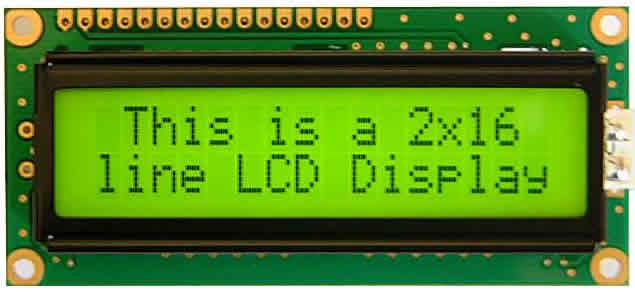
\includegraphics[width=0.8\textwidth]{overview/images/lcd.jpg}
}

%----------------------------------------------------------------------------------------
%	Character LCD pins with 1 Controller SUBESCTION
%----------------------------------------------------------------------------------------

\subsection{Character LCD pins with 1 Controller}
\centerline{
	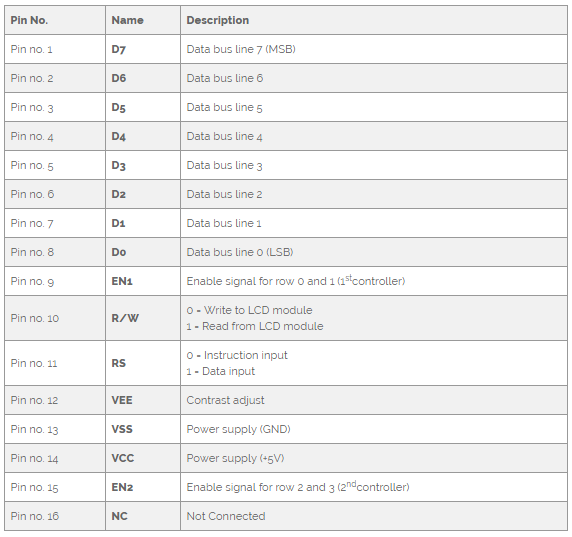
\includegraphics[width=0.8\textwidth]{overview/images/character.png}
}



